\def\theTopic{Reading 4}


\begin{center}
{\bf {\large Extra Sensory Perception}}
\end{center}

In the next classroom activity, we will look at an experiment conducted to see
if a person could read another's mind. 

 In the 1930's Dr.~J.B.~Rhine at Duke University designed experiments
to see if some undergraduate students could tell which card (see the
five ``Zener'' cards below) a ``sender'' was looking at. The deck of
cards (5 of each type) was shuffled and a card drawn at random. After
each attempt, the card was returned to the deck and the deck was
reshuffled (we call this sampling with replacement).  Therefore each
of the five card types has an equal chance of occurring at any draw.
\begin{center}
  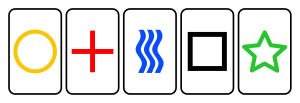
\includegraphics[width=.5\linewidth]{../plots/Zener_cards.png}
\end{center}

 Rhine found one exceptional subject in his extrasensory perception
 (ESP) research, Adam Linzmayer, an economics undergraduate at Duke.
 Linzmayer went through the experiments in 1931, and correctly
 identified 36\% of 25 cards as the ``receiver'' in the study. 

We will use Rhine's data, but we want you to know that research into ESP
(also called the ``psi'' effect) has continued.

  Go to this blog and read the Skeptic's report on recent ESP
  research.\\
  \url{https://skeptoid.com/episodes/4348}\vspace{1cm}


  Pay particular attention to how the researchers designed the
  experiment to remove all possible forms of communication between the
  individuals.  \vspace{1cm}


  What is the ``file drawer'' effect?\vspace{1cm}

  What does the author find refreshing and unique about researchers
  studing the ganzfeld effect?\vspace{1cm}



\newpage

In the next activity, we will use a spinner to generate random outcomes. 

To prepare for that, We'd like you to use the circle below (divided
 into 25 equal parts) to  build a ``Wheel of Fortune'' (just like on
 the game show)  with the following chance of each outcome:

\begin{tabular}{l|r}
Outcome & Chance\\ \hline
\$2500  & .04\\
\$1000  & .08\\
\$900  & .12\\
\$800  & .08\\
\$700  & .12\\
\$650  & .08\\
\$600  & .08\\
\$550  & .08\\
\$350  & .08\\
\$100 & .04\\
\$1 million & .02\\
Bankrupt  & .10\\
free play & .04\\
Lose a turn& .04\\
\hline
\end{tabular}
\begin{minipage}{.70\linewidth}
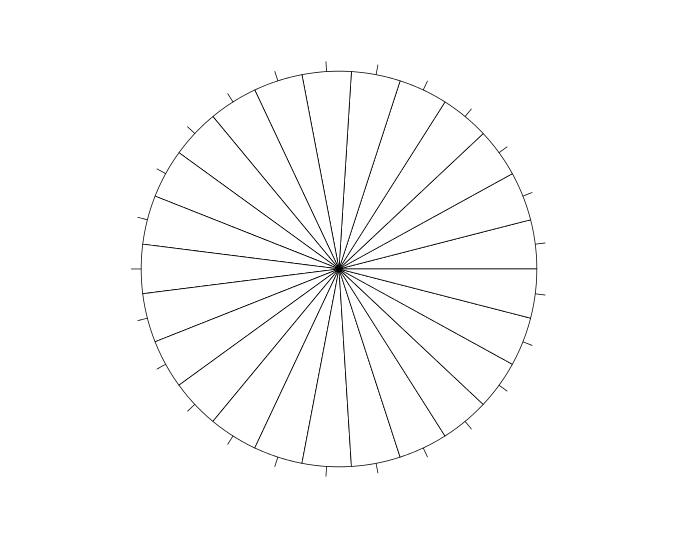
\includegraphics[width = 6in]{../plots/wheelOfFortune.png}
\end{minipage}

In the game show, they mix the outcomes up and give them different
colors. It's fine if you want to do that, but we really want you to
practice getting the right proportions, so putting, for example, all
the \$900 wedges together is fine.


\begin{center}
  {\large\bf Important Points}
\end{center}
\begin{enumerate}
\item How could the ganzfeld experiment go wrong if the scientists
  were not very careful? \vfill

\item What was the chance the subject would -- just by chance --  pick
  the right object (or video) when given the choices?\vfill 

\item On the real ``Wheel of Fortune'' do all outcomes have the same
  chance of getting picked by the pointer when the wheel stops?
\end{enumerate}


